\ifx\allfiles\undefined
\documentclass{XDBAthesis}
\def\pictures{}
\begin{document}
\else
\fi
\chapter{软件实现与实验结果}
在第四章中提到了图像处理的基本方法与预处理方法,并且提及了手势特征的提取,本章将详细讲解算法在Android平台的实现并展示实验结果。

\section{算法总体设计}

本算法分为三个模块,手势检测模块、手势分割模块和手势识别模块,图\ref{fg:chart}显示了本算法软件设计的流程图。
\begin{figure}
    \centering
    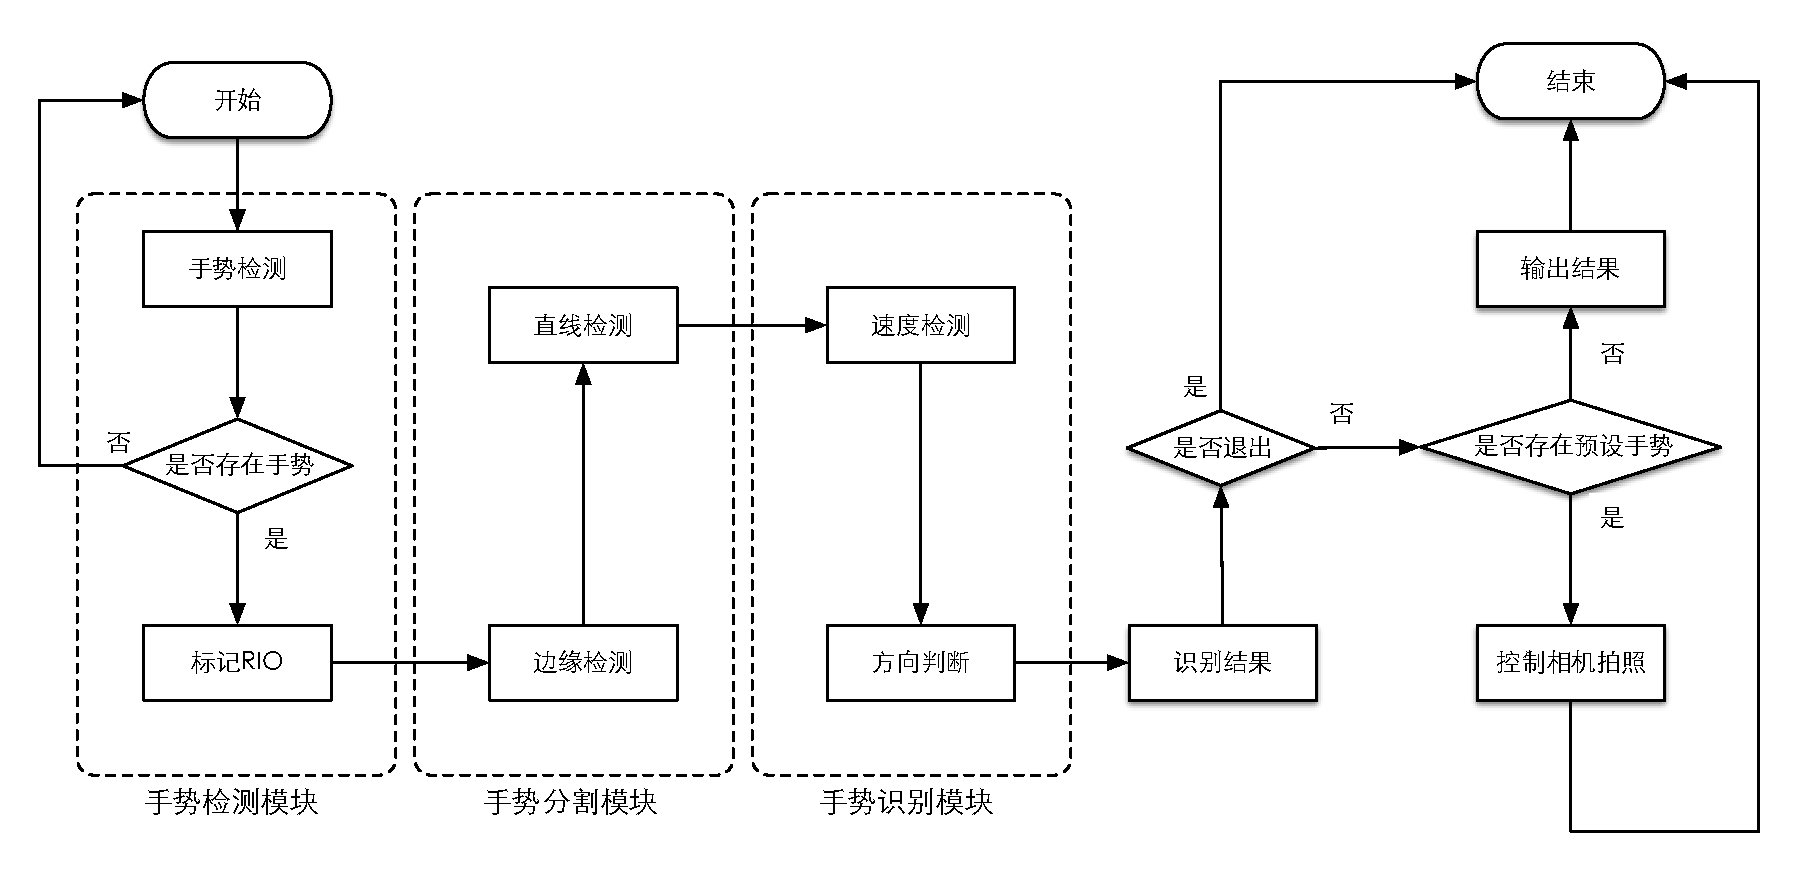
\includegraphics[width=0.9\textwidth ]{figure/chart}
    \caption{算法流程图}
    \label{fg:chart}
\end{figure}

在手势检测模块,实时检测视频流中的手势,标记检测到手势的区域为感兴趣区域;然后将感兴趣区域送入手势分割模块,利用直线检测对感兴趣区域进行处理,接着进行边缘检测和直线检测,得到手掌侧面的特征手势;在手势识别模块,对采集到的特征手势的运动进行判断,并增加时间限制,将对应的手势分别采取相对的处理机制。

\section{模块具体实现}

\subsection{手势检测模块}

功能实现使用Java语言利用OpenCV库编写了一个实时检测摄像头采集的视频流中手势的程序,抓取图片后进行灰度处理,当检测到手势时进入下一模块。

本实验是在较为复杂的背景下进行实验的,图中存在较多背景物体,同时有人脸存在,这些都没有影响到手势的正确检测,实验中仍然取得了很好的检测效果。

\subsection{手势分割模块}

    本算法采用的分割算法分为两个步骤:边缘检测和直线检测。将灰度处理过的图片采用Canny边缘检测算法,由于图片可能处理过仍有噪声,但是但是除手部以外的其他背景基本上完全滤除了,手掌形象也是清晰的。再采用直线检测,得到最终可识别的手势特征。

\subsection{手势识别模块}

在手势分割模块得到手势特征后,以移动距离为X轴,在单位时间内观察手势的运动走势并规定一定的速度范围内,手势动作最靠近哪种,就属于哪种手势识别,然后由上下左右动作分别对应指定的指令功能。
\section{软件运行结果展示}
我们利用本算法开发了个简单拍照demo,其主要功能是检测手动作,并进行相应操作:上划放大,下划缩小,左划倒计时3s拍照,右划倒计时5s拍照。
\subsection{手势识别在OpenCV上的实现}
图\ref{fg:1}为算法后台运行的log。可见,我们的算法采用间接抓取的方式,以16FPS的频率抓取图片,并处理展示。当识别到相应手势时现在log中显示,再进行相应操作。
\begin{figure}[htb]
    \centering
    \includegraphics[width=0.5\textwidth ]{figure/opencvframe}%
    \includegraphics[width=0.5\textwidth ]{figure/gesture}
    \caption{log记录}
    \label{fg:1}
\end{figure}
\subsection{CPU与系统内存占用}
CPU与系统内存占用如图\ref{fg:2}所示。可见,本算法对内存及计算量的要求并不算高,可以实际运用。
\begin{figure}[htb]
    \centering
    \includegraphics[width=0.5\textwidth ]{figure/cpu}%
    \includegraphics[width=0.5\textwidth ]{figure/memory}
    \caption{CPU与内存消耗占比图}
    \label{fg:2}
\end{figure}
\subsection{手势捕捉与处理}
当手势被识别后,进行对应功能处理。如果进入拍照功能,在屏幕右上角显示倒计时3秒,并在倒计时结束时拍照。如果是放大或缩小功能,由于前置摄像头无法实现物理变焦,故采用数字放大/缩小实现该功能。因为识别为动态过程,不方便截图展示,因此我们只截取了一个识别到左划手势并开始拍照倒计时的界面,和一个拍照完成的提示。如图\ref{fg:3}所示。
\begin{figure}[htb]
    \centering
    \includegraphics[width=0.3\textwidth ]{figure/recognize}%
    \includegraphics[width=0.3\textwidth ]{figure/capture}
    \caption{手势识别演示}
    \label{fg:3}
\end{figure}

%经过实验,我们可知在准确度,速度,稳定性上本算法均以达到实用标准。本算法已具有实际使用的可行性。

\ifx\allfiles\undefined
%\bibliographystyle{unsrt}
\bibliography{main}
\end{document}
\fi